\section{Visualize EEG signals}
    To have a nice overview between the dataset before and after remove noise, we should visualize the signal the signal first. We can also visualize the dataset with traditional tool like Matplotlib. However, Matplotlib basically just draw the dataset. Fortunately, MNE-Python is a powerful tool help us to mark the bad-channels, interact with the signal and a easier look at the very first before we apply any filter as well as afterward. 
    
    MNE-Python supports a lot of digital formats of EEG signal but the format that we have is not available in library. However, MNE give us the option to create the "raw" MNE signal file from scratch with other file format such as .csv or .tdt. First, we have to create a basic information about the structure of the signal we about to input. We have 19 electrodes so according to that, we have 19 members in the channel names.
    
    \begin{lstlisting}
        channel_names = ['FP1', 'FP2', 'F3', 'F4', 'C3', 'C4', 'P3', 'P4', 'O1', 'O2', 'F7', 'F8', 'T3', 'T4', 'T5', 'T6', 'Fz', 'Cz', 'Pz']
        sfreq = 240
        info = mne.create_info(channel_names, sfreq) 
    \end{lstlisting}
    
    In here, we have the information of the name of all electrodes that we have with the frequency of 240Hz. after import the basic information as well as the data itself we now can create the raw data of the signal with the EEGsignalValues is the data.
    
    \begin{lstlisting}
    raw = mne.io.RawArray(EEGsignalValues, info)
    \end{lstlisting}
    
    \begin{figure}
    \centering
    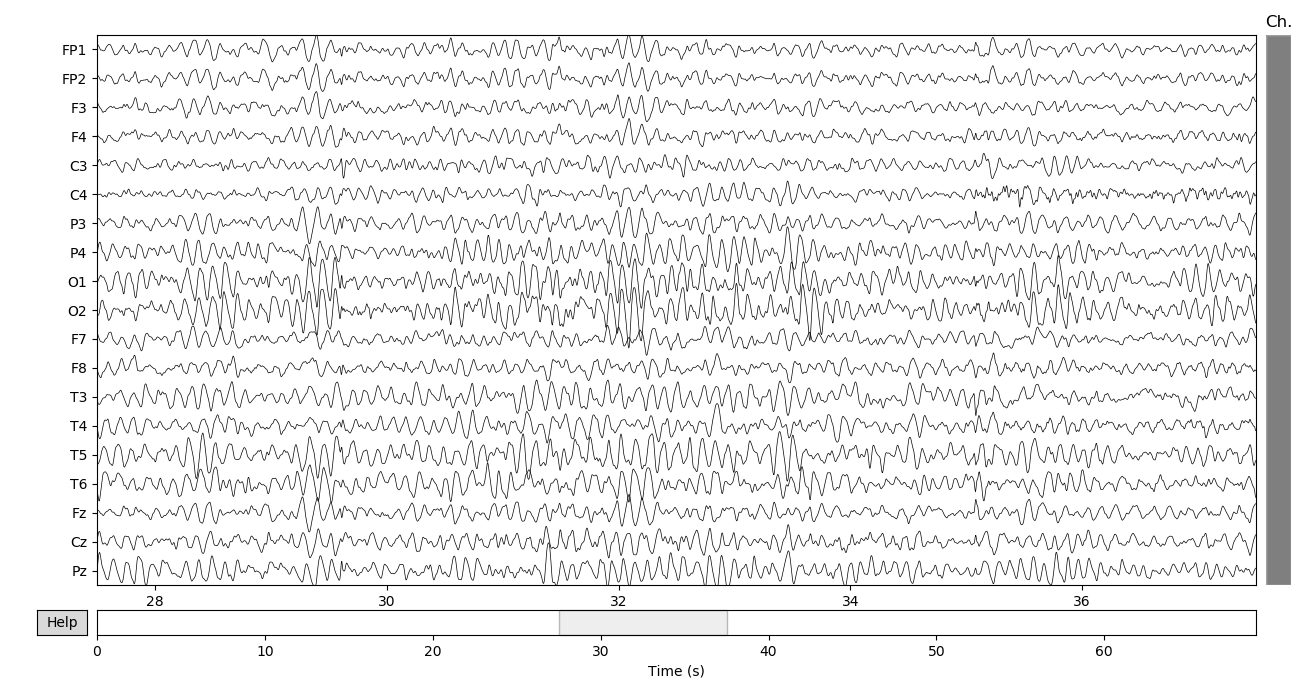
\includegraphics[width = 0.9\textwidth]{images/EEG_with_MNE.png}
    \caption{Visual EEG signal with MNE-python}
    \label{fig:visualEEGwithMNE}
    \end{figure}
    
    The result of the MNE-tool is shown in the figure 3.1. In here, we have the information of the name of all electrodes that we have with the frequency of 240Hz. after import the basic information as well as the data itself we now can create the raw data of the signal.
    
\section{Noise reduction}
    There are a lot of technique can be apply on the raw signal to remove the outliers that exist in our data. We have some of the very famous technique. The EEG signal only contain some of the frequency, and any signal that below that or above that should be remove from the signal. 
    We can deal with it by apply high-pass filter and low-pass filter. However, in our specific datasets, we will use a popular method to detect and remove outliers and it is called Z-score outliers detection.
    
    Z-score is a numerical measurement, indicates how many standard deviations an element is from the mean\cite{z_score}. The formular to caculate the score is below.

    $$z={{x-\mu}  \over \sigma }$$
    
    % $$\mid x\lfloor \sigma \rfloor \lfloor k \rfloor - \mu \lfloor k \rfloor\mid < \mid \alpha\delta^2 \mid$$

    The bigger the score is, the further the point is compare with the mean of the whole data set. If the Z-score of a point consider far enough from the mean, it is considered as an outlier. In this case, I want to consider around 5 percent of the signal as artifacts. Thus, any data point that have the Z-score over 3 and less than -3 will be removed from signal.
    
    \begin{figure}[h]
        \centering
        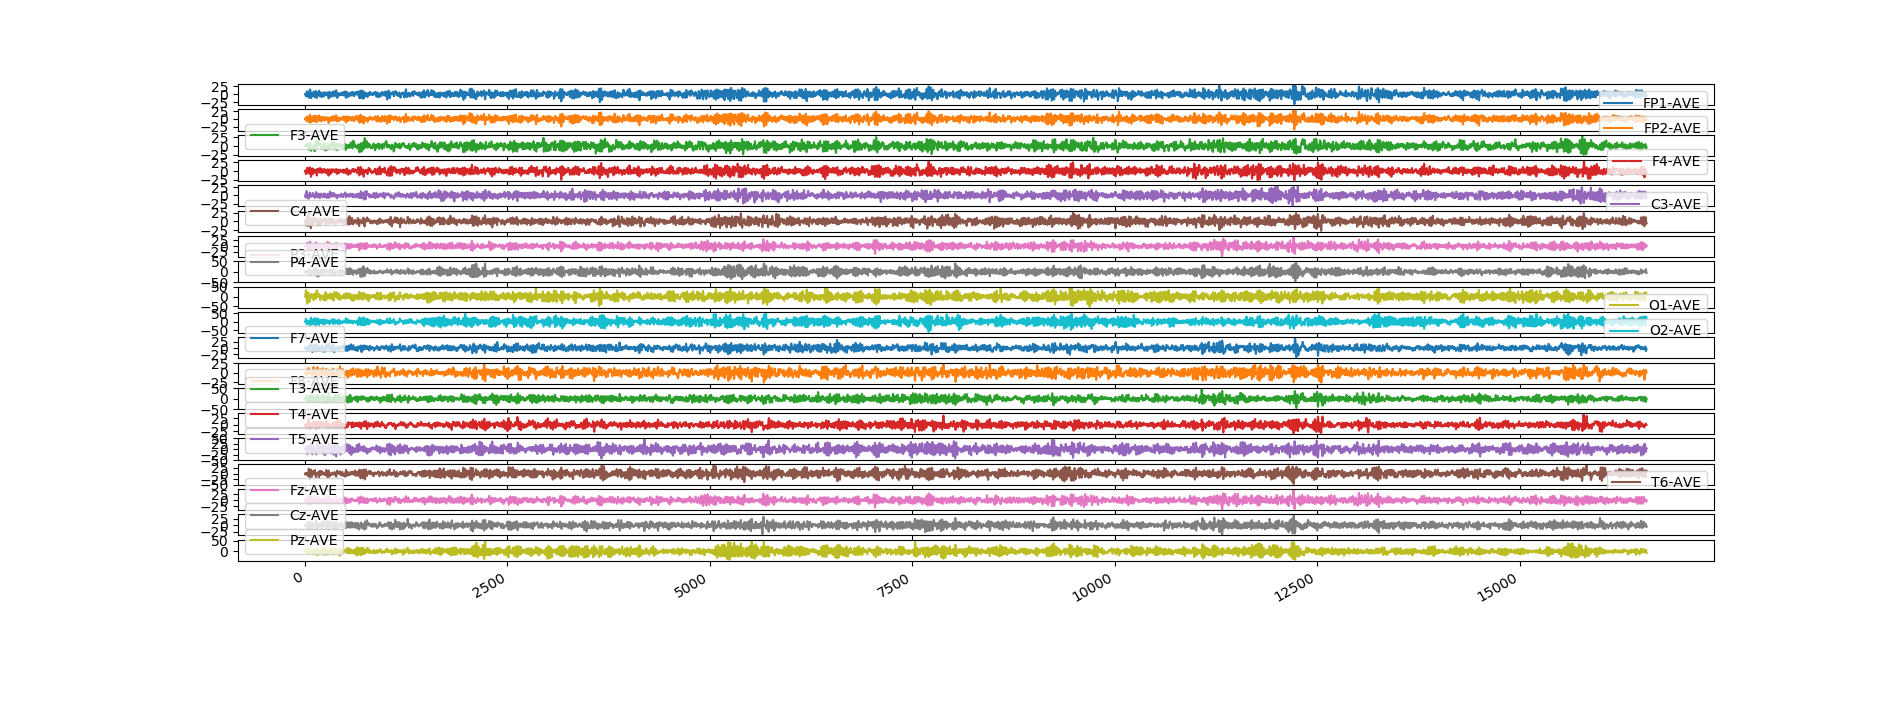
\includegraphics[width = 0.7\textwidth]{images/OriginalData.png}
        \caption{Original data}
        \label{fig:original_data}
    \end{figure}
    
    Figure~\ref{fig:original_data} is the visualized data of the signal before any impact. However, this is too small to show any changes has been made by the filter so we will only focus on a example of the FP1 signal. On the figure~\ref{fig:compare} is the electrode FP1 only. You can notice that there is some changes that applied here.
    
    \begin{itemize}
    \item Blue line: before apply Z-score
    \item Orange line: after apply Z-score
    \end{itemize}
    
    \begin{figure}[h]
        \centering
        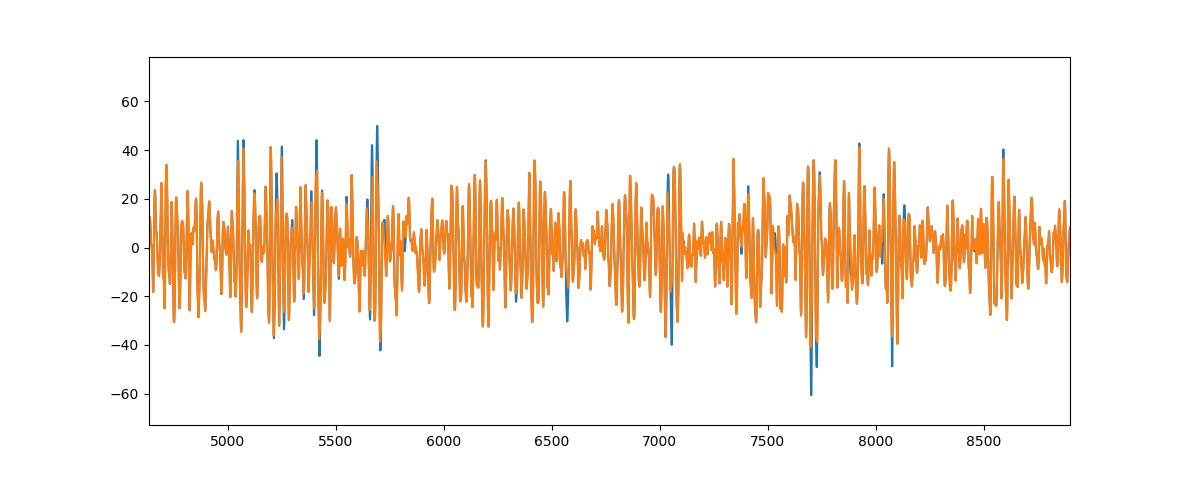
\includegraphics[width = 1\textwidth]{images/fp1-2.png}
        \caption{A part of FP1 before and after apply Z-score}
        \label{fig:compare}
    \end{figure}
    
    More closer look.
    
    \begin{figure}[h]
        \centering
        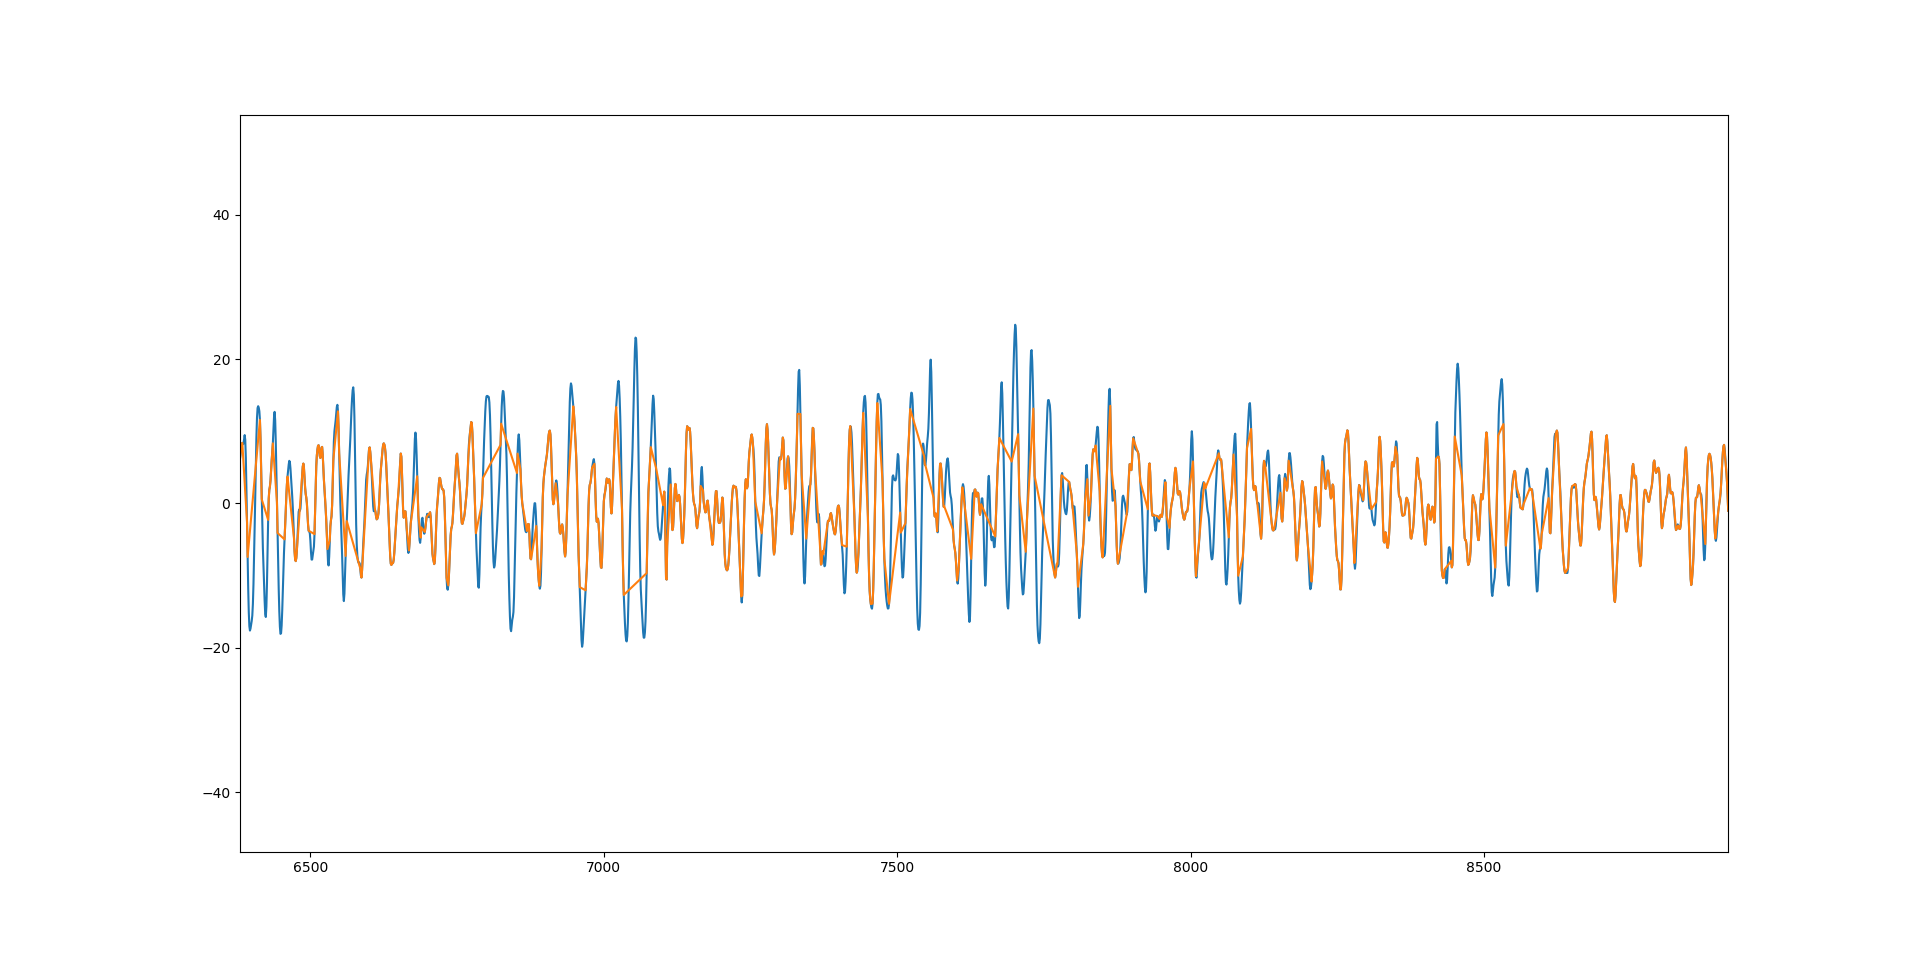
\includegraphics[width = 1\textwidth]{images/closer.png}
        \caption{Closer look at signal recorded by the electrode FP1 }
        \label{fig:closer}
    \end{figure}
    
    You can see that there is some boundary has been made all over the signal. the removed outliers around 5.7 percent of the dataset. This technique to reduce noise in the data is still not wipe all the noise but it is the most efficient technique.
    
    In the future, we can do some research about how to remove other artifact that is very hard to remove and cannot do this by normal filter. That is EOG signal and ECG signal, affected when we blinking or when our heart beating.